\titre{Solution matérielle :} Le processus indique au CPU d'ignorer les interruptions. 
	\begin{itemize}
		\item Avantage : Plus de préemption imposée
		\item Inconvénients : Cette méthode est très dangereuse, elle compromet tout le système et exige de stopper tous les CPU.
	\end{itemize}

\titre{Solution logicielle 1 : L'alternance stricte} Variable "verrou" et attente active. Attention : "Test and Modify" ne marche pas. \\
\begin{minipage}{0.5\linewidth}
Algo A : \\
\\
Tantque vrai faire\\
  //section non critique\\
	Tantque verrou != 0 faire \\
		rien \\
	Fin Tantque\\
	verrou $\leftarrow$ 1\\
Fin Tantque\\
\end{minipage}
\begin{minipage}{0.5\linewidth}
Algo B : \\
\\
Tantque vrai faire\\
  //section non critique\\
	Tantque verrou != 1 faire \\
		rien \\
	Fin Tantque\\
	verrou $\leftarrow$ 0\\
Fin Tantque\\
\end{minipage}

\begin{itemize}
	\item Avantage : Simple, purement logiciel
	\item Inconvénient : Alternance stricte (pb résolu par Peterson), forte consommation CPU
\end{itemize}

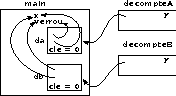
\includegraphics[width=200px]{fig7.pdf}
